\section{提案} \label{section:proposal}

本論では,Unikernel の \rr を効率的に行う \emph{VampOS}を紹介する.
VampOS の設計目標は以下のとおりです.

\begin{itemize}
    \item \textbf{Unikernel レイヤのみの Reboot-based Recovery.}{\sysname は,従来の Unikernel の再起動とは異なり,アプリケーションのメモリの内容を保持したまま Unikernel のメモリを若返らせる.アプリケーションは,私たちの Unikernel の再起動に渡って,継続して動作することができる.}
    \item \textbf{特定の Unikernel の構成に依存しない.}{特定の Unikernel のコンポーネントを対象とする \rr のメカニズムは,Unikernel の構成がアプリケーションごとに異なるため,合理的ではない.私たちのアプローチは,どのような Unikernel のコンポーネントにも適用できる.}
    \item \textbf{ダウンタイムをできるだけ短くする.}{\sysname は Unikernel の再起動によるアプリケーションのダウンタイムをできる限り短縮する.}
\end{itemize}

\begin{figure}[t]
    \begin{center}
      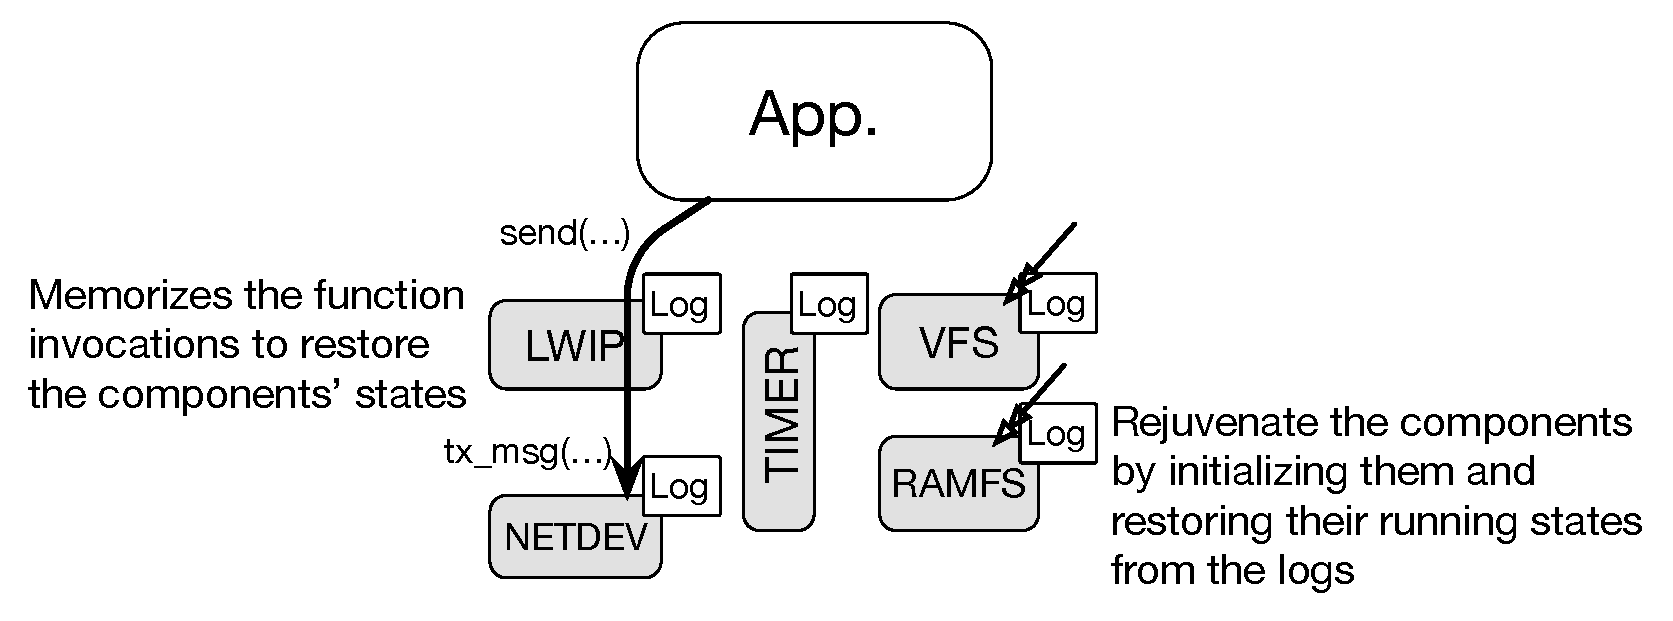
\includegraphics[scale=0.3]{./img/vampos.eps}
      \caption{\textbf{Overview of {\sysname}.} \textit{{\sysname} はコンポーネント単位での Unikernel の若返りを可能にする.そのために,\sysname は,各コンポーネントにより明確に定義され,公開されている関数をフックし,若返らせたコンポーネントの動作状態を復元するために関数呼び出しを記録する.}}
      \label{fig:overview}
    \end{center}
\end{figure}

これらの目標を達成するために,\sysname は Unikernel のカスタマイズ性を利用している.
Unikernel は多数のコンポーネントを提供し,
コンポーネント間のインタフェースが明確に定義されているため,
アプリケーションの動作に必要なコンポーネントのみを選択することができる.
\sysname の全体像を図\ref{fig:overview}に示す.
\sysname はコンポーネント単位での Unikernel の若返りを可能にし,
リンクしたアプリケーションを継続して実行できるように,
若返りしたコンポーネントの動作状態を復元する.
特に,\sysname は,公開されているコンポーネントインタフェースをフックすることにより,コンポーネント間のインタラクションを記録し,
ログを再生することで,状態を持つコンポーネントの動作状態を復元する.
例えば,ファイルシステムの若返りにおいては,\sysname は,
他のコンポーネントの動作状態の変更しないように,
そのコンポーネントのみを再起動し,若返りしたコンポーネント内部でログを再生する.

\sysname の目標は,\rr の効果を得ることであり,通常の再起動との完全な互換を目指しているものではない.
Unikernel を若返りのために,Unikernel がリンクしたアプリケーションの再起動の代わりに \sysname の再起動することができる.
\sysname のメカニズムは,
通常の再起動によるソフトウェアアップデートや再構成のような他の目的に適用するものではなく,
そのような目的のためには,通常の再起動が使われる.

\sysname の設計は以下の技術的な課題を提示する.
どのように,Unikernel をコンポーネント単位で若返らせるのか?
どのように,対象のコンポーネントのみを復元するのか?
どのように,若返りしたコンポーネントの状態を効率良く復元するのか?
次の章では,これらの課題に対する解決策を述べる.
以下の議論は Unikraft~\cite{KuenzerEtAl-Unikraft} 上のプロトタイプの開発に基づくものであるが,
IncludeOS~\cite{BratterudEtAl-IncludeOS} のような他の Unikernel にも十分に適用できる一般性を持つであろう.
